% Created 2024-07-29 Mon 16:37
% Intended LaTeX compiler: pdflatex
\documentclass[letterpaper, 12pt]{article}
\usepackage[utf8]{inputenc}
\usepackage[T1]{fontenc}
\usepackage{graphicx}
\usepackage{longtable}
\usepackage{wrapfig}
\usepackage{rotating}
\usepackage[normalem]{ulem}
\usepackage{amsmath}
\usepackage{amssymb}
\usepackage{capt-of}
\usepackage{hyperref}
\usepackage{minted}
\usepackage{xcolor}
\usepackage{hyperref}
\usepackage{tocloft}
\usepackage{minted}
\usemintedstyle{manni}
\usepackage{pdfpages}
\usepackage{fancyhdr}
\usepackage{graphicx}
\usepackage[top=1.4in, left=0.5in, right=0.5in, bottom=0.8in]{geometry}
\usepackage[T1]{fontenc}
\usepackage{helvet}
\pagestyle{fancy}
\renewcommand{\headrulewidth}{0pt}
\renewcommand{\footrulewidth}{0pt}
\setlength{\parindent}{0em}
\setlength{\parskip}{1em}
\usepackage{hyperref}
\usepackage {color}
\usepackage {tabularray}
\usepackage{xcolor}
\hypersetup{
colorlinks=true,
linkcolor=blue,
filecolor=magenta,
urlcolor=cyan,
citecolor=green,
pdfborder={0 0 0}
}
\usepackage[most]{tcolorbox}
\author{Hilduara Abreu}
\date{\today}
\title{Use of Electronic Devices School Policy\\\medskip
\large Policy regarding the use of electronic devices by students}
\hypersetup{
 pdfauthor={Hilduara Abreu},
 pdftitle={Use of Electronic Devices School Policy},
 pdfkeywords={},
 pdfsubject={},
 pdfcreator={Emacs 29.4 (Org mode 9.6.15)}, 
 pdflang={English}}
\begin{document}

\fancyfoot[C]{\setlength{\unitlength}{1in}\begin{picture}(5,0)\put(-1.8,-0.5){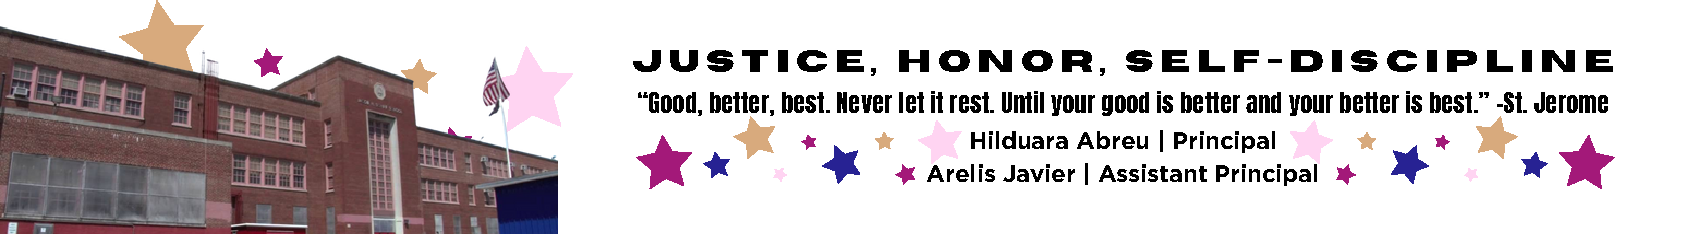
\includegraphics[width=8.8in,height=1.3in]{logo-1}}\end{picture}}
\fancyhead[C]{\setlength{\unitlength}{1in}\begin{picture}(5,0)\put(-1.9,-0.5){
\includegraphics[width=8.9in,height=1.3in]{logo-2}}\end{picture}}
\fancyhead[R]{\thepage}
\pagenumbering{gobble}

\begin{document}
\vspace*{0.01in}
\tcbuselibrary{}
\newtcolorbox{bluebox}[1][]{
  colback=blue!5!white,
  colframe=blue!75!black,
  fonttitle=\bfseries,
  coltitle=black,
  enhanced,
  attach boxed title to top center={yshift=-2mm},
  title=#1,
  boxed title style={colback=blue!50!white}
}
\newtcolorbox{greenbox}[1][]{
  colback=green!5!white,
  colframe=green!75!black,
  fonttitle=\bfseries,
  coltitle=black,
  enhanced,
  attach boxed title to top center={yshift=-2mm},
  title=#1,
  boxed title style={colback=green!50!white}
}
\newtcolorbox{redbox}[1][]{
  colback=red!5!white,
  colframe=red!75!black,
  fonttitle=\bfseries,
  coltitle=black,
  enhanced,
  attach boxed title to top center={yshift=-2mm},
  title=#1,
  boxed title style={colback=red!50!white}
}

\section*{Table of Contents}
\label{sec:org7ae2a0b}
\begin{enumerate}
\item \hyperref[sec:org817b2ae]{Introduction}
\item \hyperref[sec:org9c0dafd]{English Version}
\item \hyperref[sec:org5778b94]{Versión en Español}
\end{enumerate}
\pagebreak
\vspace*{-1cm}

\section*{Introduction}
\label{sec:org817b2ae}
Dear Parents and School Community,

Welcome to PS 192! We are committed to providing a safe and nurturing environment where every student can thrive academically, socially, and emotionally. As we embark on another exciting school year, it is essential for all members of our school community to stay informed about our policies, rules, events, and core values. These guidelines help us create a positive and productive learning atmosphere for our students.

At PS 192, we believe in the power of education to transform lives. Our dedicated staff works tirelessly to offer the highest quality education, empowering our students to become the next generation of thinkers and leaders who will make a positive impact on our city and beyond. Your partnership and support are crucial in this journey, and we thank you for being an integral part of our community.

Together, we can ensure that PS 192 continues to be a place where every child feels valued and inspired to reach their full potential. We look forward to a successful and enriching school year with your continued involvement and cooperation.

With Justice, Honor, and Self-Discipline,


\includegraphics[width=0.2\textwidth]{hil_signature}

\textbf{Hilduara Abreu, Principal}

\textbf{The school of Joyful Learning!}

\href{www.ps192.org}{www.ps192.org}
\pagebreak
\vspace*{-1cm}

\section*{English Version}
\label{sec:org9c0dafd}
Date: \href{https://www.ps192.org}{September 5th, 2024}

Subject: \textbf{Use of Electronic Devices}

\begin{redbox}[PS 192 | Policy]
Prohibited Devices
Although not recommended, students are allowed to bring the following electronic items to school:
\begin{itemize}
\item Cell phones
\item Portable music and entertainment systems (e.g., iPods, MP3 players)
\end{itemize}
\textit{The student and/or parent is responsible for the safety and security of these devices. The school does not provide facilities to charge devices.}
\vspace*{3mm}

Important Key Points:
\begin{itemize}
\item Before 8:00 AM or after 3:35 PM in any location within the school where it does not disrupt educational activities.
\item Be turned on or used during instructional time, except for educational purposes with the teacher's approval.
\item Be turned on or used during quizzes, tests, or exams unless explicitly authorized or as part of an Individualized Education Program (IEP) or Section 504 Accommodation Plan.
\item Be in the possession of students during the school's bell schedule.
\item Be turned on or used during fire drills or other emergency preparedness exercises.
\item Be used in bathrooms.
\item Be used during lunch in the cafeteria or schoolyard.
\item Be used between classes in hallways and stairwells.
\end{itemize}
\end{redbox}

Use of electronic devices must comply with the DOE’s Discipline Code, school policy, Chancellor’s Regulation A-413, and the DOE’s Internet Acceptable Use and Safety Policy (IAUSP).
\pagebreak
\vspace*{-0.5cm}

\textbf{\textbf{Violations and Disciplinary Actions}}

Violations of this policy may result in:
\begin{itemize}
\item Confiscation of the device, with return only to the parent/legal guardian after a behavioral conference.
\item Revocation of the privilege to bring electronic items to school.
\item Additional disciplinary measures in accordance with the DOE Discipline Code.
\end{itemize}

With Justice, Honor, and Self-Discipline,


\includegraphics[width=0.2\textwidth]{hil_signature}

\textbf{Hilduara Abreu, Principal}

\textbf{The school of Joyful Learning!}

\href{www.ps192.org}{www.ps192.org}
\pagebreak
\vspace*{-1cm}

\section*{Versión en Español}
\label{sec:org5778b94}
Fecha: \href{https://www.ps192.org}{5 de septiembre de 2024}

Asunto: \textbf{Uso de Dispositivos Electrónicos}

\begin{greenbox}[PS 192 | Política]
Dispositivos Prohibidos
Aunque no se recomienda, se permite a los estudiantes traer los siguientes artículos electrónicos a la escuela:
\begin{itemize}
\item Teléfonos móviles
\item Sistemas portátiles de música y entretenimiento (por ejemplo, iPods, reproductores MP3)
\end{itemize}
\textit{El estudiante y/o los padres son responsables de la seguridad de estos dispositivos. La escuela no proporciona instalaciones para cargar dispositivos.}
\vspace*{3mm}

Puntos Clave Importantes:
\begin{itemize}
\item Antes de las 8:00 AM o después de las 3:35 PM en cualquier lugar dentro de la escuela donde no interrumpa las actividades educativas.
\item Encenderse o utilizarse durante el tiempo de instrucción, excepto para fines educativos con la aprobación del maestro.
\item Encenderse o utilizarse durante exámenes, pruebas o evaluaciones, a menos que esté explícitamente autorizado o como parte de un Programa de Educación Individualizado (IEP) o Plan de Acomodación de la Sección 504.
\item Estar en posesión de los estudiantes durante el horario de timbre de la escuela.
\item Encenderse o utilizarse durante simulacros de incendio u otros ejercicios de preparación para emergencias.
\item Utilizarse en los baños.
\item Utilizarse durante el almuerzo en la cafetería o el patio escolar.
\item Utilizarse entre clases en los pasillos y escaleras.
\end{itemize}
\end{greenbox}

El uso de dispositivos electrónicos debe cumplir con el Código de Disciplina del DOE, la política escolar, el Reglamento del Canciller A-413 y la Política de Uso Aceptable de Internet y Seguridad del DOE (IAUSP).
\pagebreak
\vspace*{-0.5cm}

\textbf{\textbf{Violaciones y Acciones Disciplinarias}}

Las violaciones de esta política pueden resultar en:
\begin{itemize}
\item Confiscación del dispositivo, con devolución solo al padre/tutor legal después de una conferencia de comportamiento.
\item Revocación del privilegio de traer artículos electrónicos a la escuela.
\item Medidas disciplinarias adicionales de acuerdo con el Código de Disciplina del DOE.
\end{itemize}

Con Justicia, Honor y Autodisciplina,


\includegraphics[width=0.2\textwidth]{hil_signature}

\textbf{Hilduara Abreu, Directora}

\textbf{¡La escuela del Aprendizaje Alegre!}

\href{www.ps192.org}{www.ps192.org}
\end{document}
